\chapter*{Практика 2. Помехоустойчивое кодирование}
\addcontentsline{toc}{chapter}{Практика 2. Помехоустойчивое кодирование}
\label{ch:2_practice}
\label{sec:fig}
    

{ \itshape
    \textbf{Задание:}  Реализовать операцию сверточного кодирования и витербидекодирования битового сообщения.
}    
\begin{figure}[ht]
    \centering
    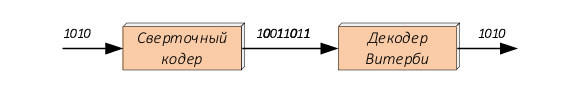
\includegraphics[width=0.8\textwidth]{convolutional_encoder_decoder.png}
    \caption{Блоксхема работы свёрточного кодера и декодера Витерби}
    \label{fig:symbolic_encoder_decoder.png}
\end{figure}

{
    \textbf{}

}
\begin{figure}[ht]
    \centering
    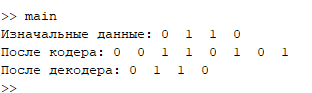
\includegraphics[width=0.8\textwidth]{2practice_result.png}
    \caption{Результат второй практики}
    \label{fig:2practice_result.png}
\end{figure}

\endinput